\documentclass{article}
\usepackage[utf8]{inputenc}
\usepackage{geometry}
 \geometry{
 a4paper,
 total={170mm,257mm},
 left=20mm,
 top=20mm,
 }
 \usepackage{graphicx}
 \usepackage{titling}
 \usepackage{graphicx}
\usepackage{amsmath}
\usepackage{esint}
  
\DeclareMathOperator{\sech}{sech}
\DeclareMathOperator{\cosec}{cosec}
\DeclareMathOperator{\cosech}{cosech}


 \title{Assignment \textbf{2} (Lecture 6-8)
}
\author{Syed Suhaib Ahmad}
\date{\today}
 
 \usepackage{fancyhdr}
\fancypagestyle{plain}{%  the preset of fancyhdr 
    \fancyhf{} % clear all header and footer fields
    
    \fancyfoot[C]{1}
    \fancyhead[L]{8.02x - Electricity and Magnetism}
    \fancyhead[R]{\theauthor}
}
\makeatletter
\def\@maketitle{%
  \newpage
  \null
  \vskip 1em%
  \begin{center}%
  \let \footnote \thanks
    {\LARGE \@title \par}%
    \vskip 1em%
    %{\large \@date}%
  \end{center}%
  \par
  \vskip 1em}
\makeatother

\usepackage{lipsum}  
%\usepackage{cmbright}

\begin{document}

\maketitle


\subsubsection*{Problem 2.1 - Electric field of a point charge inside a hollow metallic sphere}
A hollow metallic sphere is initially uncharged. Now imagine that a positive concentrated charge $q$ is placed somewhere (not in the middle) inside the sphere without touching the walls.
\begin{figure}[h]
        \centering
        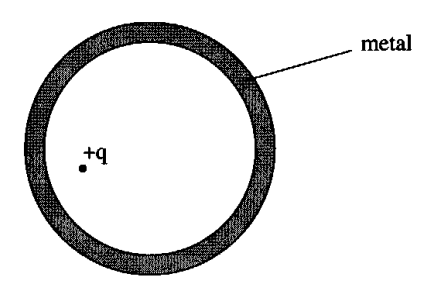
\includegraphics[width=0.35\linewidth]{figs/fig_prob_2.1.png}
       % \caption{Caption}
        %\label{fig:enter-label}
    \end{figure}
\begin{enumerate}
    \item[(a)]Qualitatively, what is the charge distribution on the inner surface of the metal and what is it on the outer surface? 
    \item[(b)]Suppose that you move the charge $q$ around inside the cavity. Does the charge distribution on the outer surface of the sphere change? Explain your answer.
    \item[(c)]You now bring the point charge $q$ in contact with the inner surface of the sphere. What is the charge distribution then on the inner surface and on the outer surface?
\end{enumerate}
\textbf{Solution(a)}
\\
\\Initially all the charge resides uniformly on the outer surface of the metal. However, upon placing a test charge $+q$ somewhere inside the metal, an induced charge would show up on the inside surface of the metal to counter the electric field due to $+q$, leaving a charge $q_{\text{outside}}$ on the outside surface of the metal. This happens because the net electric field inside the surface of a conductor is always zero. This very fact also helps us in realizing that the induced charge, $q_{\text{induced}}$ inside the metal is actually equal to $-q$. Now for the charge distribution outside the metal, we can use the law of conservation of charge and since the metal was initially electrically neutral, we get
\[q_{\text{outside}}+q_{\text{induced}}=0\Rightarrow q_{\text{outside}}=-q_{\text{induced}}=+q.\]
It is also crucial to note that the surface charge is still uniformly distributed as the electric field inside the metal is zero and consequently the metal is an equipotential surface. Finally, we can conclude that electric field outside the metal at any point has only one solution: $\frac{+q}{4\pi\epsilon_0r^2}$ and any other solution would be contradictory to everything stated so far.
\\
\\\textbf{Solution(b)}
\\
\\The outer charge distribution will remain constant in the given scenario due to reasons mentioned in (a). Moreover, we are merely changing the position of the test charge inside the metal and consequently the distribution of inner charge.
\\
\\\textbf{Solution(c)}
\\
\\This would result in a very dense induced charge distribution at the point of contact to cancel all the effects of charge $+q$, leaving the same amount of surface charge calculated in (a) and its corresponding electric field. Again, we only changed the position of inner charge inside the metal, which has no effect on the surface charge.  

\subsubsection*{Problem 2.2 - Electric field and potential of a charged cylinder}
Consider a very long cylinder of radius $a$ with its axis along the $z-$axis of a cartesian coordinate system. The cylinder is uniformly charged; its constant volume charge density is $\rho$ (positive).
\begin{enumerate}
\item[(a)]Using symmetry arguments show that $\Vec{\boldsymbol{E}}$ should be radial both inside and outside the cylinder.
\item[(b)]Using Gauss' Law find the magnitude of $\Vec{\boldsymbol{E}}$ as a function of $r$, for $0\leq r\leq a$, and for $r>a$. Do the two results match at $r=a$?
\item[(c)]Using answers in part (b) calculate the potential difference, $\Delta V$, between a point at a distance $r$ from the $z-$axis and a point on the $z-$axis.
\end{enumerate}
\textbf{Solution(a)}
\\
\\Due to the cylindrically symmetric charge distribution, the electric field vector can only point in the direction that is radial. If we suppose that the electric field is in a nonradial direction, it would make an unacceptable distinction between the upper and lower portions of the cylinder; the cylinder is infinitely long and the uniform charge distribution has no reason to prefer either of the +$z$ or $-z$ direction.
\\
\\\textbf{Solution(b)}
\\
\\Using the arguments from part (a), it can be concluded that the electric field is of constant magnitude over a concentric path around the cylinder, thus, we consider a Gaussian surface in the form of a cylinder of Radius $r$ and length $l$. For the case $0\leq r\leq a$, the total charge enclosed by the Gaussian surface is $Q_{\text{enc}}=\rho\pi r^2l$. It is also important to note that electric flux through the two circular surfaces of our Gaussian surface is zero due to the radial nature of electric field ($\Vec{\boldsymbol{E}}\cdot d\Vec{\boldsymbol{A}}=0$).
\[\oiint\Vec{\boldsymbol{E}}\cdot d\Vec{\boldsymbol{A}}=\frac{Q_{\text{enc}}}{\epsilon_0}\Rightarrow E\times2\pi rl=\frac{\rho\pi r^2l}{\epsilon_0}\Rightarrow E=\frac{\rho r}{2\epsilon_0}\]
Similarly, for $r>a$, the same method is used, but this time the charge enclosed by our Gaussian surface is the total charge on the cylinder ($Q_{\text{total}}=\rho\pi a^2l$).
\[E\times2\pi rl=\frac{\rho\pi a^2l}{\epsilon_0}\Rightarrow E=\frac{\rho a^2}{2\epsilon_0r}.\]
If $r=a$ is substituted in both of the cases, we get the same result $E=\frac{\rho a}{2\epsilon_0}$.
\\
\\\textbf{Solution(c)}
\\
\\The potential difference between 0 and $r$ ($r\leq a)$ is
\[\Delta V=-\int_{0}^{r}\Vec{\boldsymbol{E}}\cdot d\Vec{\boldsymbol{l'}}=-\int_{0}^{r}E(r')\boldsymbol{\hat{r}}\cdot \boldsymbol{\hat{r}}dr'=-\int_{0}^{r}\frac{\rho r'}{2\epsilon_0}\,dr'=-\frac{\rho r^2}{4\epsilon_0}.\]
For $r>a$, we break the integral into two parts
\[\Delta V=-\int_{0}^{a}\frac{\rho r'}{2\epsilon_0}\,dr'-\int_{a}^{r}\frac{\rho a^2}{2\epsilon_0r'}\,dr'=-\frac{\rho a^2}{4\epsilon_0}-\frac{\rho a^2}{2\epsilon_0}(\ln r-\ln a)=-\frac{\rho a^2}{4\epsilon_0}\left(1+2\ln\frac{r}{a}\right).\]

\subsubsection*{Problem 2.3 - Electric field, Potential, and Electrostatic Potential Energy}
At each corner of a cube of side $l$ there is a point charge $Q$.
\begin{enumerate}
    \item[(a)] What is the potential at the center of the cube ($V=0$ at $r=\infty$)?
    \item[(b)] What is the potential at each corner due to the other seven charges?
    \item[(c)]What is the total potential energy of this system?
\end{enumerate}
\textbf{Solution(a)}
\\
\\The center of cube means that the coordinates of this point about any corner are $(l/2,l/2,l/2)$. Thus the distance of this point from either of the eight corners is $d=\sqrt{(l/2)^2+(l/2)^2+(l/2)^2}=\sqrt{3}l/2$. Hence we can apply the superposition principle to find the electric potential due to all eight charges residing at each of the corners of the cube.
\[V_\text{center}=\frac{Q_{\text{total}}}{4\pi\epsilon_0d}=\frac{8Q}{4\pi\epsilon_0\times\frac{\sqrt{3}l}{2}}=\frac{4Q}{\sqrt{3}\pi\epsilon_0l}.\]
\textbf{Solution(b)}
\\
\\Since each corner has the exact charge as all other corners and we are dealing with a cube, electric potential at any corner would be equal to electric potential at all other corners.
\[V_{\text{corner}}=\frac{1}{4\pi\epsilon_0}\left(\frac{3Q}{l}+\frac{3Q}{\sqrt{2}l}+\frac{Q}{\sqrt{3}l}\right)\approx(5.7)\frac{1}{4\pi\epsilon_0}\frac{Q}{l}.\]
\textbf{Solution(c)}
\\
\\Total potential energy of this system is work done to assemble all the eight charges in their respective positions assuming that each of these charges were initially at infinity. This might seem very trivial to calculate but if we look closely, this can become a bit non-intuitive and bizarre. For example, the work needed to move first charge $Q_1$ from infinity to one of the corners of the cube would be zero as the cube is initially uncharged and there is no electric field. However, bringing in the second charge, $Q_2$, requires work as the first charge opposes the coming of the second charge, we call this work $W_{12}$. So, according to this pattern, we would have to add many terms as the work on each new charge would increase due to previously added charges and thus the total potential energy would be
\[E_p=W_{12}+W_{13}+W_{23}+W_{14}+W_{24}+W_{34}+. . .+ W_{ij}=\frac{1}{2}\sum_{r=1}^{i}\sum_{u=1}^{j}\frac{Q_rQ_u}{4\pi\epsilon_0d_{ru}}\]
Fortunately, we do not need to calculate the above summation as we have already calculated an important quantity that would be helpful in finding the solution to this problem. If we multiply the value of $V_{\text{corner}}$ (electric potential due to seven charges) with $4Q$, the obtained value is the total electrostatic potential energy of all the eight charges. It is important to note that the value of $V_{\text{corner}}$ is not multiplied with $8Q$ as it would count all the number of pairs twice. 
\[E_p=\frac{1}{2}QV_{\text{corner}}=(22.8)\frac{1}{4\pi\epsilon_0}\frac{Q^2}{l}.\]

\subsubsection*{Problem 2.4 - Electric field, Potential, and Electrostatic Potential Energy}
Point charges $Q_1$ ($+5\mu$\,C), $Q_2$ ($-1\mu$\,C), and $Q_3$ ($+2\mu$\,C) reside on three corners of a square with sides 1\,m; the distance from $Q_2$ to $P_3$ is 2\,m.
\begin{enumerate}
    \item[(a)]What is the electric potential, $V$, in $P_1$, $P_2$, and $P_3$? (Normalize the potential to be zero at $\infty$).
    \item[(b)]Are their points or surfaces in space (other than infinity) where $V$ is zero? 
    \item[(c)]There are two points where the electric field equals zero. Could you guess approximately where these points are? State your reasons.
    \item[(d)]What is the electrostatic potential energy of the system?
    \item[(e)]Suppose we release the three charges so that they can move freely in empty space. How much energy is released in the form of kinetic energy? Does it matter in what sequence one releases the charge?
    \begin{figure}[h]
        \centering
        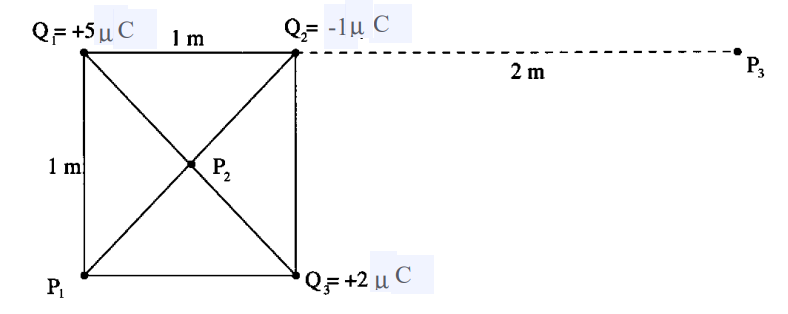
\includegraphics[width=0.7\linewidth]{figs/fig_prob_2.4.png}
       % \caption{Caption}
        %\label{fig:enter-label}
    \end{figure}
\end{enumerate}
\textbf{Solution(a)}
\\
\\Electric potential, $V(r)$, at any point $r$ can be computed using the superposition principle.
\[V(\boldsymbol{\Vec{r}})=\frac{1}{4\pi\epsilon_0}\left(\frac{Q_1}{|\boldsymbol{\Vec{r}}-\boldsymbol{\Vec{r_1}}|}+\frac{Q_2}{|\boldsymbol{\Vec{r}}-\boldsymbol{\Vec{r_2}}|}+\frac{Q_3}{|\boldsymbol{\Vec{r}}-\boldsymbol{\Vec{r_3}}|}\right)=\frac{10^{-6}}{4\pi\epsilon_0}\left(\frac{5}{|\boldsymbol{\Vec{r}}-\boldsymbol{\Vec{r_1}}|}-\frac{1}{|\boldsymbol{\Vec{r}}-\boldsymbol{\Vec{r_2}}|}+\frac{2}{|\boldsymbol{\Vec{r}}-\boldsymbol{\Vec{r_3}}|}\right).\]
$P_1$:
\[V(\boldsymbol{\Vec{r}})=\frac{10^{-6}}{4\pi\epsilon_0}\left(\frac{5}{1}-\frac{1}{\sqrt{2}}+\frac{2}{1}\right)=5.7\times10^4\,\text{V}.\]
$P_2$:
\[V(\boldsymbol{\Vec{r}})=\frac{10^{-6}}{4\pi\epsilon_0}\left(\frac{5}{0.5\sqrt{2}}-\frac{1}{0.5\sqrt{2}}+\frac{2}{0.5\sqrt{2}}\right)=7.6\times10^4\,\text{V}.\]
$P_3$:
\[V(\boldsymbol{\Vec{r}})=\frac{10^{-6}}{4\pi\epsilon_0}\left(\frac{5}{3}-\frac{1}{2}+\frac{2}{\sqrt{5}}\right)=1.9\times10^4\,\text{V}.\]
\textbf{Solution(b)}
\\
\\As we can see, the system consists of three charges; $+5\mu\,$C, $-1\mu\,$C and $+2\mu\,$C. So, it is quite clear that there is a region close to the negative charge where the term $\frac{1}{|\boldsymbol{\Vec{r}}-\boldsymbol{\Vec{r_2}}|}$ gets much bigger in magnitude that it cancels out the other two terms resulting in a net electric potential of zero.
\\
\\\textbf{Solution(c)}
\\
\\There are two points where the electric field is, one between the two positive charges and the other is at right of the negative charge. First point appears between two positive charges (closer to $Q_3$) because both charges exert a repulsive force on each other and hence there comes a point where both force cancels out producing zero electric field. The other point appears on the upper right of $Q_2$ as both of the positive charges are on left of $Q_2$, thus at this point the outward forces due to $Q_1$ and $Q_3$ are balanced by the inward force of $Q_2$. 
\\
\\\textbf{Solution(d)}
\\
\\The total electrostatic potential energy of the system is the work done on each of the charges $Q_1$, $Q_2$ and $Q_3$ to bring them from infinity to their locations described in the problem. Thus, we can add the individual electrostatic potential energies of each pair of charges to obtain the net.
\[E_p=\frac{1}{4\pi\epsilon_0}\left(\frac{Q_1Q_2}{|\boldsymbol{\Vec{r_1}}-\boldsymbol{\Vec{r_2}}|}+\frac{Q_1Q_3}{|\boldsymbol{\Vec{r_1}}-\boldsymbol{\Vec{r_3}}|}+\frac{Q_2Q_3}{|\boldsymbol{\Vec{r_1}}-\boldsymbol{\Vec{r_3}}|}\right)=\frac{10^{-12}}{4\pi\epsilon_0}\left(\frac{-5}{1}+\frac{10}{\sqrt{2}}-\frac{2}{1}\right)=6.4\times10^{-4}\,\text{J}.\]
\textbf{Solution(e)}
\\
\\If all charges are released at once in such a manner that they all end up at infinity, the sum of their respective kinetic energies would be equal to the value calculated in (d). However, due to the different polarities and magnitudes of charges, they would not always end up at infinity and thus their kinetic energies would vary according to the final arrangement of system. For example, if we release $Q_2$ first, it would be attracted by $Q_1$ due to its greater magnitude and opposite nature and eventually it would find itself revolving around $Q_1$. In the meantime, releasing $Q_3$ might well be enough to take it to infinity but it depends on which moment in time is $Q_3$ released. In conclusion, the sequence in which the charges are released does matter indeed and there are possibly an infinite number of solutions to the final position and kinetic energies of the individual charges.

\subsubsection*{Problem 2.5 - Electric potential of a flat ring with hole in its center}
A thin flat nonconducting disk, with radius $R_0$ and charge
$Q$, has a hole with a radius $R_0/2$ in its center. Find the electric potential $V(x)$ at points along the symmetry $(x)$ axis of
the disk (a line perpendicular to the disk, passing through its
center). Let $V = 0$ at $x = \infty$.
\\
\\\textbf{Solution}
\\
\\The area  of this disk is $A=\pi R_0-\pi\left(\frac{R_0}{2}\right)^2=\frac{3\pi R_0^2}{4}$. Hence we can calculate the surface charge density to be $\sigma=\frac{4Q}{3\pi R_0^2}$. Now we consider an infintesimal ring of radius $r$ and width $dr$. The charged carried by the ring is $dq=\sigma(2\pi r\,dr)$. The electric potential due to this ring at a perpendicular distance of $x$ from the symmetry axis of the disk is 
\[dV(x)=\frac{1}{4\pi\epsilon_0}\frac{dq}{\sqrt{x^2+r^2}}=\frac{1}{4\pi\epsilon_0}\frac{\sigma(2\pi r)}{\sqrt{x^2+r^2}}\,dr.\]
Integrating from $r=\frac{R_0}{2}$ to $r=R_0$ gives the total electric potential of the disk.
\[V(x)=\frac{\sigma}{2\epsilon_0}\int_{\frac{R_0}{2}}^{R_0}\frac{r}{\sqrt{x^2+r^2}}\,dr=\frac{2Q}{3\pi\epsilon_0R_0^2}\int_{\frac{R_0}{2}}^{R_0}\frac{d}{dr}\left(\sqrt{x^2+r^2}\right)\,dr\]
\[V(x)=\frac{2Q}{3\pi\epsilon_0R_0^2}\left[\sqrt{x^2+R_0^2}-\sqrt{x^2+\frac{R_0^2}{4}}\right].\]

\subsubsection*{Problem 2.6 - Electric breakdown fields}
Under standard conditions of temperature and pressure, dry air will break down (i.e, lose its insulating quality), and sparking will result when the electric field exceeds about $3\times10^6$\,V/m.
\begin{enumerate}
\item[(a)]Suppose that we wish to maintain an isolated metallic sphere at $-4000$\,V. What is the minimum radius of the sphere for which there is no sparking?
\item[(b)]At this minimum radius, what is the total charge on the radius?
\item[(c)]Now consider a free electron in the air, very near the charged sphere. If the electron is initially at rest, what radial distance will it travel before reaching a kinetic energy of $10$\,eV? Assume that no collision with the air molecules takes place during this interval of time.
\item[(d)]Compare your answer in (c) with the typical electron mean-free path in the air which is about $10^{-6}$\,m. 
\end{enumerate}
\textbf{Solution(a)}
\\
\\Let $r$ be the radius of the metallic sphere. We know that electric potential and electric field are given by the expressions
\[V=\frac{1}{4\pi\epsilon_0}\frac{Q}{r}\,\,\,\,\,\,\,\,\,\,E=\frac{1}{4\pi\epsilon_0}\frac{Q}{r^2}\]
respectively. Thus we can relate both quantities as $E=\frac{V}{r}$. Upon substituting the values we get
\[3\times10^6=\frac{4000}{r}\Rightarrow r=\frac{4000}{3\times10^6}=1.33\times10^{-3}\,\text{m}.\]
Hence the minimum distance for which there is no sparking is $1.33$\,mm.
\\
\\\textbf{Solution(b)}
\\
\\From part (a), $Q=4\pi\epsilon_0rV=4\pi\epsilon_0\times1.33\times10^{-3}\times-4000=-5.9\times10^{-10}\,$C.
\\
\\\textbf{Solution(c)}
\\
\\An electron near the surface of the sphere will be accelerated away from the sphere due its negative polarity. Assuming that the electric field is constant through the electron's journey
\[eEl=\frac{1}{4\pi\epsilon_0}\frac{eQ}{r}\Rightarrow eEl=10e\Rightarrow l=\frac{10}{3\times10^6}=3.33\times10^{-6}\,\text{m}.\]
This value of $l$ justifies our assumption of constant electric field as $E\geq 3\times10^6\,$V/m for $l\leq1.33\times10^{-3}\,$m.
Moreover, the electric field falls off as $\frac{1}{r^2}$ but for this value of $l$ it falls of an insignificant amount.
\\
\\\textbf{Solution(d)}
\\
\\From the information given in (d), we can conclude that an electron gains 10\,eV within approximately three mean-free paths.
The energy required to ionize an air molecule is 10\,eV, so if the electric field is greater than $3\times10^6$, the electron will have enough energy to ionize an air molecule and thus one more electron will be released in air, which might ionize another air molecule and eventually a chain reaction of ionization will start resulting in a discharge through air from the sphere.   

\subsubsection*{Problem 2.7 - 1.33\,keV charges}
An electron starting from rest acquires $1.33$\,keV of
kinetic energy in moving from point $A$ to point $B$.
\begin{enumerate}
    \item[(a)]How much kinetic energy would a proton acquire, starting from rest at $B$ and moving to point $A$? 
    \item[(b)]Determine the ratio of their speeds at the end of their respective trajectories.
\end{enumerate}
\textbf{Solution(a)}
\\
\\Let the electric field in the space is $\Vec{\boldsymbol{E}}$, which is a function of $r$ (distance from the source of field). Kinetic energy gained by the electron in its trek from point $A$ to point $B$ can be written as
\[K.E_e=-e\Delta V_{AB}=-e\left(-\int_{A}^{B}\Vec{\boldsymbol{E}}\cdot d\Vec{\boldsymbol{l}}\right)=e\int_{A}^{B}\Vec{\boldsymbol{E}}\cdot d\Vec{\boldsymbol{l}}.\]
Similarly the kinetic energy gained by the proton when it travels from $B$ to $A$ can be represented as
\[K.E_p=e\Delta V_{BA}=e\left(-\int_{B}^{A}\Vec{\boldsymbol{E}}\cdot d\Vec{\boldsymbol{l}}\right)=e\left(-\int_{A}^{B}\Vec{\boldsymbol{E}}\cdot-d\Vec{\boldsymbol{l}}\right)=e\int_{A}^{B}\Vec{\boldsymbol{E}}\cdot d\Vec{\boldsymbol{l}}=K.E_e.\]
Hence, the proton would gain the same amount of energy as electron in its respective journey, which is $1.33$\,keV.
\\
\\\textbf{Solution(b)}
\\
\\Using the standard formula for kinetic energy we have
\[\frac{1}{2}m_ev_e^2=\frac{1}{2}m_pv_p^2\Rightarrow\frac{v_e}{v_p}=\sqrt{\frac{m_p}{m_e}}=\sqrt{\frac{1.67\times10^{-27}}{9.11\times10^{-31}}}\approx42.8\,.\]

\subsubsection*{Problem 2.8 - Dropping charged objects in the earth's electric field}
Near the surface of the Earth there is an electric field of
about $150\,$V/m which points downward. Two identical balls with mass $m=0.340$\,kg are dropped from a height of
$2.00$\,m, but one of the balls is positively charged with $q_1=450\,\mu$C, and the second is negatively charged with $q_2=-450\,\mu$C. Use conservation of energy to determine
the difference in the speeds of the two balls when they hit
the ground. (Neglect air resistance.)
\\
\\\textbf{Solution}
\\
\\For this problem, we assume that both gravitational potential and electrostatic potential energies are zero at $h=0$, meaning all of the initial energy of both balls will be converted to kinetic energy as they hit the ground. Using law of conservation of energy, we have
\[m_1gh+q_1Eh=\frac{1}{2}m_1v_1^2\Rightarrow v_1=\sqrt{2gh+\frac{2q_1Eh}{m_1}}=\sqrt{2(9.81)(2)+\frac{2(450\times10^{-6})(150)(2)}{0.340}}\approx6.327\,\text{m/s}.\]
Similarly, using the same method for the second, we obtain
\[v_2=\sqrt{2gh+\frac{2q_2Eh}{m_2}}=\sqrt{2(9.81)(2)-\frac{2(450\times10^{-6})(150)(2)}{0.340}}\approx6.200\,\text{m/s}.\]
Thus, the difference in the speeds of the balls is
\[\Delta v=v_1-v_2=6.327-6.200=0.127\,\text{m/s}.\]
The above result ($v_1>v_2$) is completely intuitive as we know that positive charges travel from a higher potential to lower potential and vice versa. So, the positively charged ball is forced by the electric field to move downward while the other ball is forced to move upward against gravity.



\end{document}
